\documentclass[12pt]{report}
\setlength{\parindent}{0em}
\setlength{\parskip}{1em}

\usepackage[utf8]{inputenc}
\usepackage{graphicx}
\graphicspath{ {Figures/} }

\usepackage[a4paper,width=150mm,top=25mm,bottom=25mm]{geometry}

\usepackage{fancyhdr}
\pagestyle{fancy}

\fancyhead{}
\fancyhead[R]{\leftmark}

\usepackage{biblatex}
\addbibresource{references.bib}

\usepackage{enumitem}

\usepackage{caption}
\usepackage{subcaption}

\begin{document}

\begin{titlepage}
    \begin{center}
        \vspace{1cm}
        
        \large
        \textbf{Exploring The Integration Of Micropayements Between IoT Devices Using Blockchain And Payment Channel Technology}
        
        \vspace{1cm}
        
        
\includegraphics[width = 0.4\textwidth]{uct_logo.jpg}
        
        \vspace{1cm}
        
        \large
        Prepared By:\\ 
        \textbf{Elle Mouton}\\
        \textbf{(MTNELL004)}
        
        
        \vfill 
        Prepared for: \\
        \textbf{Mr Jarryd Son} and \textbf{Assoc Prof. Amit Mishra}\\
        Department of Electrical Engineering\\
        University of Cape Town\\
        South Africa
        
        \vspace{1.5cm}
        
        11 October 2019
        
         \vspace{1.5cm}
        Submitted to the Department of Electrical Engineering at the University of Cape Town in partial fulfillment of the academic requirements for the degree of Bachelor of Science in Electrical and Computer Engineering
        
    \end{center}
\end{titlepage}


\thispagestyle{plain}
\begin{center}
    \Large
    \textbf{Abstract}
\end{center}


\newpage
\thispagestyle{plain}
\begin{center}
    \Large
    \textbf{Acknowledgements}
\end{center}


\newpage
\thispagestyle{plain}
\begin{center}
    \Large
    \textbf{Declaration}
\end{center}



\tableofcontents.
\listoffigures

\chapter{Introduction}
example of figure
\begin{figure}[h]
\centering

\includegraphics[scale=0.5]{uct_logo.jpg}
\caption{An example Image}
\label{fig:x cubed graph}
\end{figure}


\section{Background}

\section{Problem statement}

\section{Problem objectives}

\section{Scope and limitations}

\section{Plan of development}

\chapter{Literature Review}
\section{Current payments methods in IoT}

The Internet of Things (IoT) has grown rapidly over the past few years and at the end of 2018, Forbes predicted that the number of cellular IoT connections will reach 3.5 billion by 2030 \parencite{internet_forecasts}. The Internet of Things essentially allows devices connected to it, communicate with other similarly connected devices all around the world. In this sense IoT can be useful for many applications but what will significantly boost the IoT industry is the ability for devices not only to communicate but also to transact with one another.

The idea of having IoT devices perform transactions raises the question of privacy and security because IoT devices are not all held to the same standards as phones and laptops when it comes to cybersecurity. Due to this and due to consumers becoming more aware of the dangers of sharing their private banking information with devices, the IoT industry is still limited when it comes to using the IoT devices for payments \parencite{iot_light}.

The problem of security and privacy is one that must be addressed if the IoT industry is to grow to its full potential. This is due to the fact that devices constantly require and exchange things like electricity, fluid, data-streams and more. Devices either exchange these things between each other or with humans and it is often the case that these supplies must be paid for and so it is necessary for the IoT devices to be able to handle payments efficiently and securely.

An additional problem with the existing methods of payments on IoT devices is that they use fiat currencies which then requires transfers through banks and this results in many complications such as the need to provide private information and high transaction fees that make continuous micropayments expensive and inefficient. Micropayments are essential in the IoT industry due to the nature of the content being exchanges between devices. It can be concluded that for payments to work in the IoT industry, any solution requiring intermediate third-parties and discrete payments will not suffice. The IoT industry require a payment method that allows for cheap micropayments that will be secure and private on a peer-to-peer network \parencite{iot_light}.



\section{Distributed Payment Ledger Technology}

A paper named \textit{‘Micropayments Between IoT Devices: A Qualitative Study Analyzing the Usability of DLT’s in an IoT Environment’} written by Sebastian El-Hage and Gustav Holst \parencite{micro_iot_devices} outlines what Distributed Ledger Technology (DLT) is and how it could possibly facilitate micropayments in the IoT world. In this section then main findings of the paper will be presented and discussed.

The paper defines a distributed ledger as a \textit{‘database where members of a P2P network all hold the information stored within it. There exists a consensus among the entities regarding the current state of the ledger, thus all updates demand the validation of the network ’}\parencite{micro_iot_devices}. Blockchain technology is then a distributed ledger where the information shared between the peers in the network is stored in the form of blocks connected in a linked-list structure in a chronological order. The workings of a blockchain will be discussed more thoroughly in Chapter Chapter \ref{backTheory}. but for the purpose of this section it is important to know that due to the way blockchains work, how blocks are created, the way that transactions are created and verified using public key cryptography and the decentralized nature of the public blockchain, it can be mathematically shown that transactions are immutable once included in a block and that privacy and security is ensured. There are many different implementations of blockchains and two of the most popular are the Bitcoin and Ethereum blockchains.

\subsection{What blockchain offers for the IoT world}

Blockchain technology opens up new avenues for payments in the IoT industry. If each IoT device had a copy of a blockchain ledger (ex: Bitcoin Blockchain) then inter-device payments could be made securely and privately. It would also provide a more standardized communication method which then reduces the need for constant network management and maintenance \parencite{iot_dev_integration}.

\subsection{Limitations of blockchain tech in the IoT world}

Although blockchain technologies could reduce the initial problems of security and privacy in IoT payments, they does not solve the problem of enabling continuous micropayments and also introduce new problems. 
Firstly, each block in a blockchain has a size limit which results in a limit to the number of transactions that can be included in each block. Adding to this, one of the characteristics of a secure blockchain is one that makes the creation (or mining) or each block very difficult thus making it a lengthly process. For example, a block in the Bitcoin blockchain takes roughly 10 minutes to create. These size and time restrictions have resulted in Bitcoin being able to validate an average of 4.6 transactions per second \parencite{blockchain_speed}. When this figure is compared to the 1700 transactions per second that Visa can process \parencite{blockchain_speed}, it is clear that using blockchains for IoT payments will not scale well especially If continuous micropayments is the goal. 
Another concern is that blockchain requires most of the devices using it to store a complete copy of the entire ledger meaning that each device needs to store each transaction. If IoT devices used blockchain technology for micropayments, blocks would fill up quickly and the blockchain size would grow exponentially meaning that the disk size required by a device for the purpose of storing a copy of the blockchain would grow quickly. This is another scalability issue that blockchain technology introduces.
Secondly, blockchain technology still does not solve the problem of high transaction fees and so it does not provide a cost-effective solution for micropayments \parencite{micro_iot_devices}.

\subsection{Payment Channel Technology}

The paper goes on to describe a technology that uses a second layer of a main blockchain to perform transactions on (ie. Transactions are performed off-chain). Such a technology uses bi-directional payment channels between devices that are both connected to the blockchain and uses smart contracts (known as HTLCs) to set up these channels. An implementation using this technology has been developed for both the Bitcoin and Ethereum networks and these are called the Lightning Network and the Raiden Network respectively. These networks enable payments to be routed through the peer-to-peer network though an interconnection of payment channels. This means that direct channels between two interacting parties is not required. The details of the Lightning Network will be outlined in Chapter \ref{backTheory}.

\subsection{How payment channels overcome limitations of blockchain technology}

Since these payment channels are held off-chain, two parties could conduct an infinite number of transactions between them and only the final distribution of value needs to be communicated to the blockchain. This allows for near instant transactions with very low fees and requires very few transactions to be verified on-chain. The Lightning Network thus overcomes the scalability limits that pure blockchain technology has while still maintaining the benefits of security provided by the blockchain through the use of smart contracts.

\subsection{Micropayment integration into IoT}

The study concludes by reiterating that blockchain technology such as Bitcoin along with payment channel technology such as the Lightning Network are promising solutions for facilitating micropayments between IoT devices. A number of micropayment uses were also identified such as pay-per-use instead of subscription based business models so that users pay for exactly what they consume. 

The paper concludes by saying that although blockchain and payment channel technology seem to provide a sustainable way of integrating micropayments into the IoT industry, not much has been done in terms of testing any such implementations and logistical aspects of actual implementations should be tested and analysed.

\section{Different blockchain technologies}


\subsection{Bitcoin and the Lightning Network}

\subsection{Ethereum and the Raiden Network}

\section{Existing implementations}

\chapter{Background Theory} \label{backTheory}
\section{Blockchain and Bitcoin technology}

\section{Payment channels and the Lightning Network}

\chapter{Implementation}
\section{Implementation Development Plan}

In all the steps of implementation, there will be 2 entities that will need to communicate with each other through the Lightning Network. The entities will be called A and B.

For all the steps the aim will be to ensure that the two entities, A and B, can communicate in the correct way. The two activity diagrams shown below in figure \ref{fig:activity_diagrams} outline the scenarios that should be tested at each step in the development. The activity diagram in figure \ref{fig:test_1} shows the most basic form of transaction that should happen between entity A and B in which B will produce an invoice that A will then pay. The activity diagram shown in figure \ref{fig:test_2} shows a more complicated scenario where after having established an initial connection, entity A can continue to use a resource provided by B and be charged for the resource in micropayments.

\begin{figure}[h!]
     \centering
     \begin{subfigure}[b]{0.2\textwidth}
         \centering
         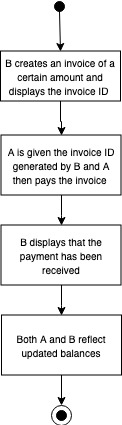
\includegraphics[width=\textwidth]{activity_1.jpg}
         \caption{Test 1}
         \label{fig:test_1}
     \end{subfigure}
     \hfill
     \begin{subfigure}[b]{0.4\textwidth}
         \centering
         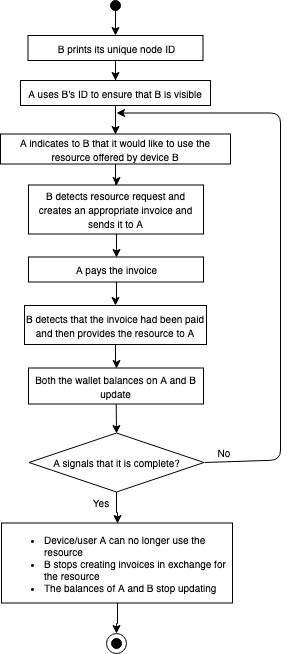
\includegraphics[width=\textwidth]{activity_2.jpg}
         \caption{Test 2}
         \label{fig:test_2}
     \end{subfigure}
     \caption{Activity diagrams showing implementation tests}
      \label{fig:activity_diagrams}
\end{figure}

\subsection{Step 1}

\begin{enumerate}[label=\alph*)]
    \item Download the Bitcoin blockchain onto a laptop computer
    \item Install and set up a Bitcoin server (bitcoind) and a Lightning Server (lnd)
    \item Create two separate Lightning wallets and instances so that it is as if two different devices on the Lightning Network exist.
    \item  Implement and test two programs that recreate the scenarios shown in the activity diagrams in figure \ref{fig:activity_diagrams}.
\end{enumerate}

\begin{figure}[h!]
\centering
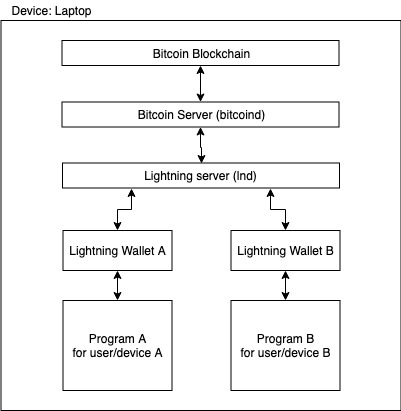
\includegraphics[scale=0.5]{Figures/step1.jpg}
\caption{Step 1 block diagram}
\label{fig:step1}
\end{figure}


\subsection{Step 2}

\begin{enumerate}[label=\alph*)]
    \item Set up Bitcoin and Lightning on a Raspberry Pi device
    \item Implement and test two programs that recreate the scenarios shown in the activity diagrams in figure \ref{fig:activity_diagrams}. (This will require manually informing device A of the Lightning node ID of device B.
\end{enumerate}

\begin{figure}[h!]
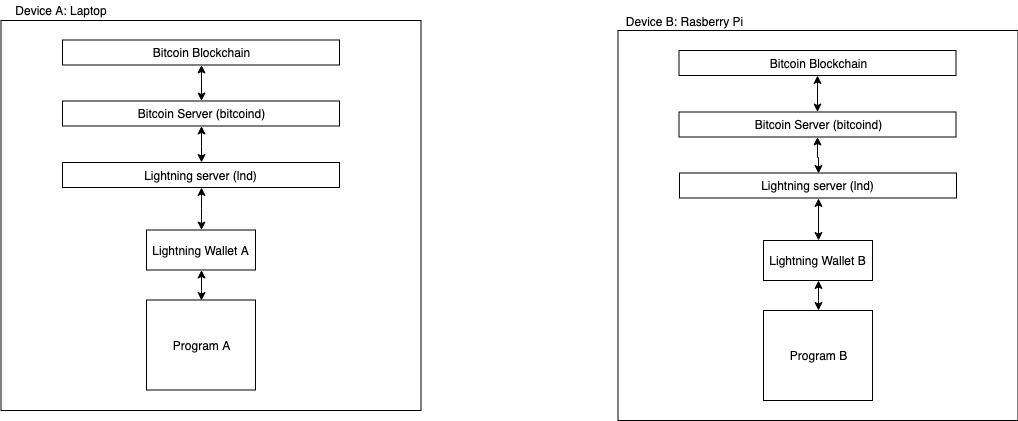
\includegraphics[scale=0.5]{Figures/step2.jpg}
\caption{Step 2 block diagram}
\label{fig:step2}
\end{figure}

\subsection{Step 3}

\begin{enumerate}[label=\alph*)]
    \item Integrate a camera and QR reader into system A
    \item Integrate a display and QR presenter into system B
    \item Implement and test two programs that recreate the scenarios shown in the activity diagrams in figure \ref{fig:activity_diagrams} but with the following developments:
        \begin{itemize}
            \item B displays its invoice/ID info on the QR display
            \item A gets B’s invoice/ID data from its camera and QR decoder
        \end{itemize}
\end{enumerate}

\begin{figure}[h!]
\centering
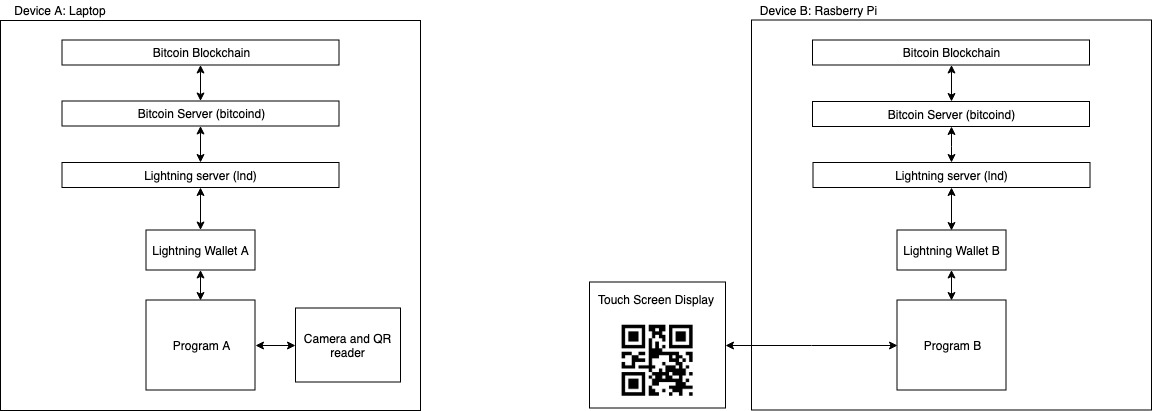
\includegraphics[scale=0.5]{Figures/step3.jpg}
\caption{Step 3 block diagram}
\label{fig:step3}
\end{figure}

\subsection{Step 4}

\begin{enumerate}[label=\alph*)]
    \item Add details such as a user interface for both A and B
    \item Add a potentiometer and configure its input to represent the amount of the resource that A is using and ensure that B creates invoices with amounts based on the potentiometer reading.
    \item Add an LED as a way for B to show that its resource is or is not currently available to A.
\end{enumerate}

\begin{figure}[h!]
\centering
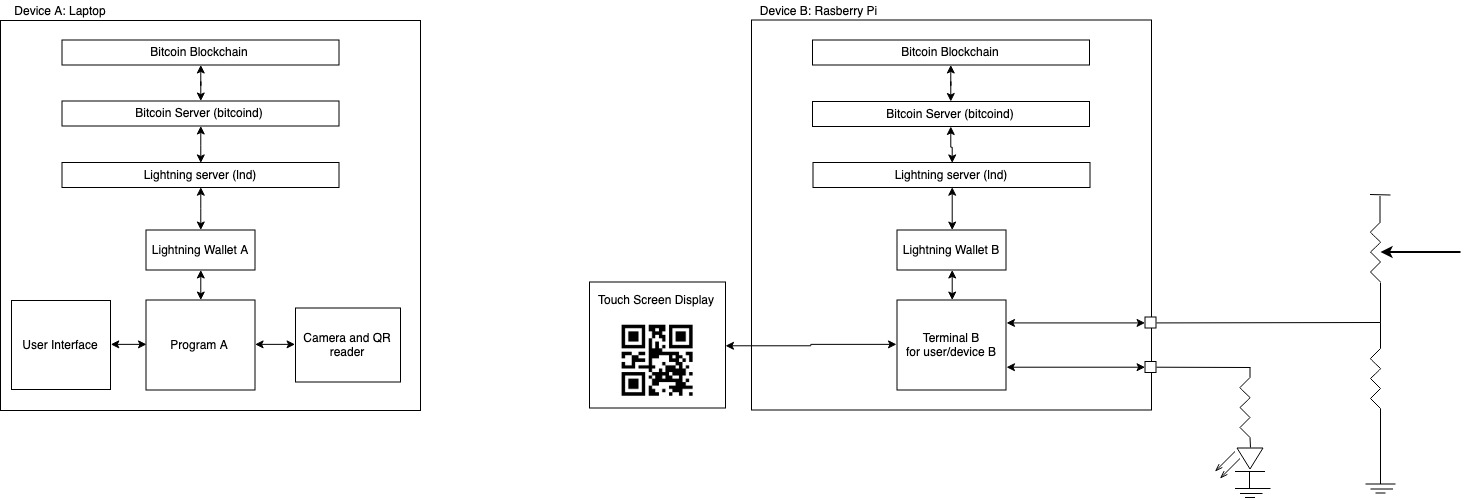
\includegraphics[scale=0.5]{Figures/step4.jpg}
\caption{Step 4 block diagram}
\label{fig:step4}
\end{figure}

\chapter{Results}
\input{Chapters/results.tex}

\chapter{Discussion}
\input{Chapters/discussion.tex}

\chapter{Conclusions}
\input{Chapters/conclusions.tex}

\chapter{Recommendations}
\input{Chapters/recommendations.tex}

\appendix
\chapter{Appendix}
\input{Chapters/appendix.tex}

\printbibliography

\end{document}
